\section{Numerical Examples}
\begin{figure}[H]
\centering
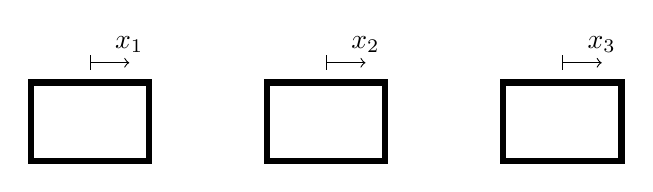
\begin{tikzpicture}
\draw[line width=.8mm](2,0)rectangle++(1.5,1);
\draw[line width=.8mm](5,0)rectangle++(1.5,1);
\draw[line width=.8mm](8,0)rectangle++(1.5,1);
\setstructmech{linewidth=.4mm}
\Spring{.5,.75}{2,.75}{1.5}
\Spring{3.5,.75}{5,.75}{1.5}
\Spring{6.5,.75}{8,.75}{1.5}
\Spring{9.5,.75}{11,.75}{1.5}
\Dashpot{6.5,.25}{8,.25}{1.5}
\Dashpot{.5,.25}{2,.25}{1.5}
\FixedSupport[-90]{.5,.5}{2}
\FixedSupport[90]{11,.5}{2}
\draw[|->](2.75,1.25)--++(.5,0)node[above]{$x_1$};
\draw[|->](5.75,1.25)--++(.5,0)node[above]{$x_2$};
\draw[|->](8.75,1.25)--++(.5,0)node[above]{$x_3$};
\end{tikzpicture}
\end{figure}